\documentclass[12pt]{article}

\usepackage[margin=1in]{geometry}
\usepackage{amsmath,amssymb}
\usepackage{graphicx}
\usepackage{enumitem}
\usepackage{draftwatermark}

\SetWatermarkText{Jiayu Chen}
\SetWatermarkScale{0.3}
\SetWatermarkAngle{45}
\SetWatermarkColor[gray]{0.9}

\title{Mathematical Analysis --- Lecture 1-4}
\author{}
\date{}

\begin{document}
\maketitle

\begin{quote}
Class 5\% \quad Homework 15\% \quad Quizzes 20\% \quad Midterm 20\% \quad Final 40\%
\end{quote}

\section*{Preliminary}
\begin{itemize}
	\item $\mathbb{N}$ denotes the set of all positive integers.
	\item $\mathbb{Z}$ denotes the set of all integers.
	\item $\mathbb{Q}$ denotes the set of all rational numbers.
	\item $\mathbb{R}$ denotes the set of all real numbers.
\end{itemize}

\section*{Limits and Continuity}

\subsection*{1. Key idea}
\begin{quote}
We use limits to describe the tendency of a function as the variable approaches a given point, but not the value at the point.
\end{quote}

\subsection*{2. Important examples}

\subsubsection*{Example 1: Same limit, different value at the point}
\[
f(x)=
\begin{cases}
x^2\sin\dfrac{1}{x},&x\ne0,\\
0,&x=0,
\end{cases}
\]
\begin{center}
	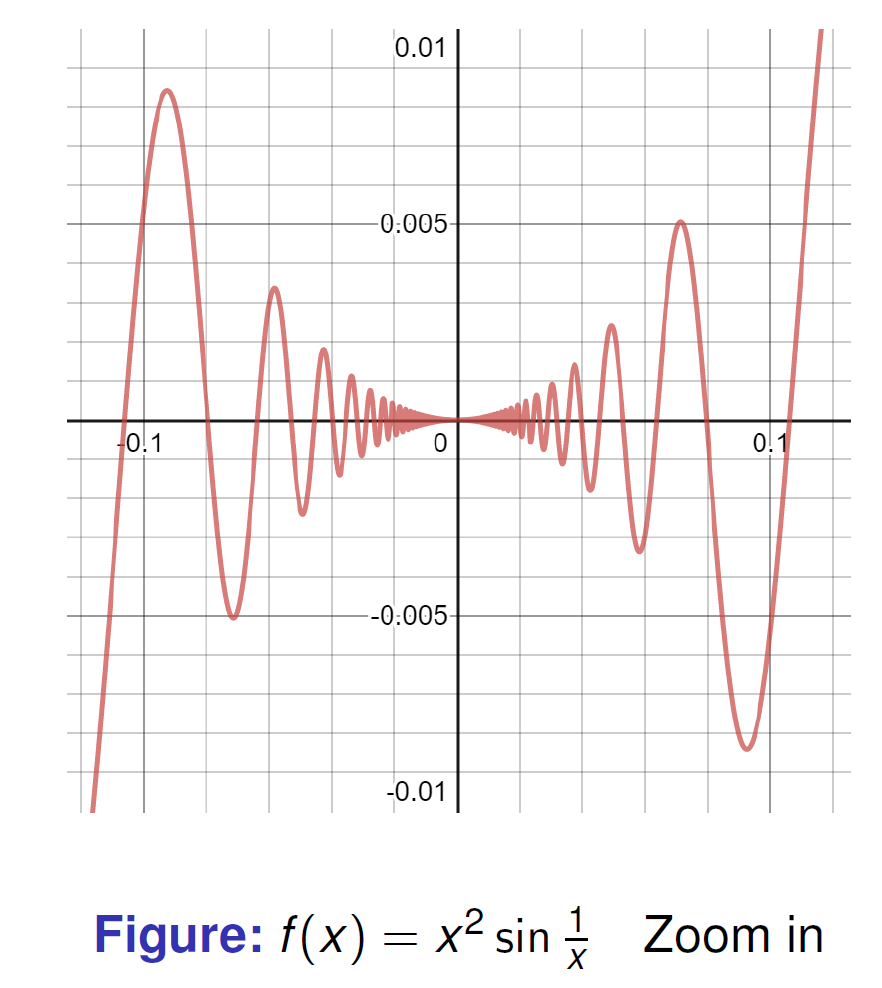
\includegraphics[width=0.65\textwidth]{image.png}
\end{center}

\[
g(x)=
\begin{cases}
x\sin\dfrac{1}{x},&x\ne0,\\
1,&x=0.
\end{cases}
\]
\begin{center}
	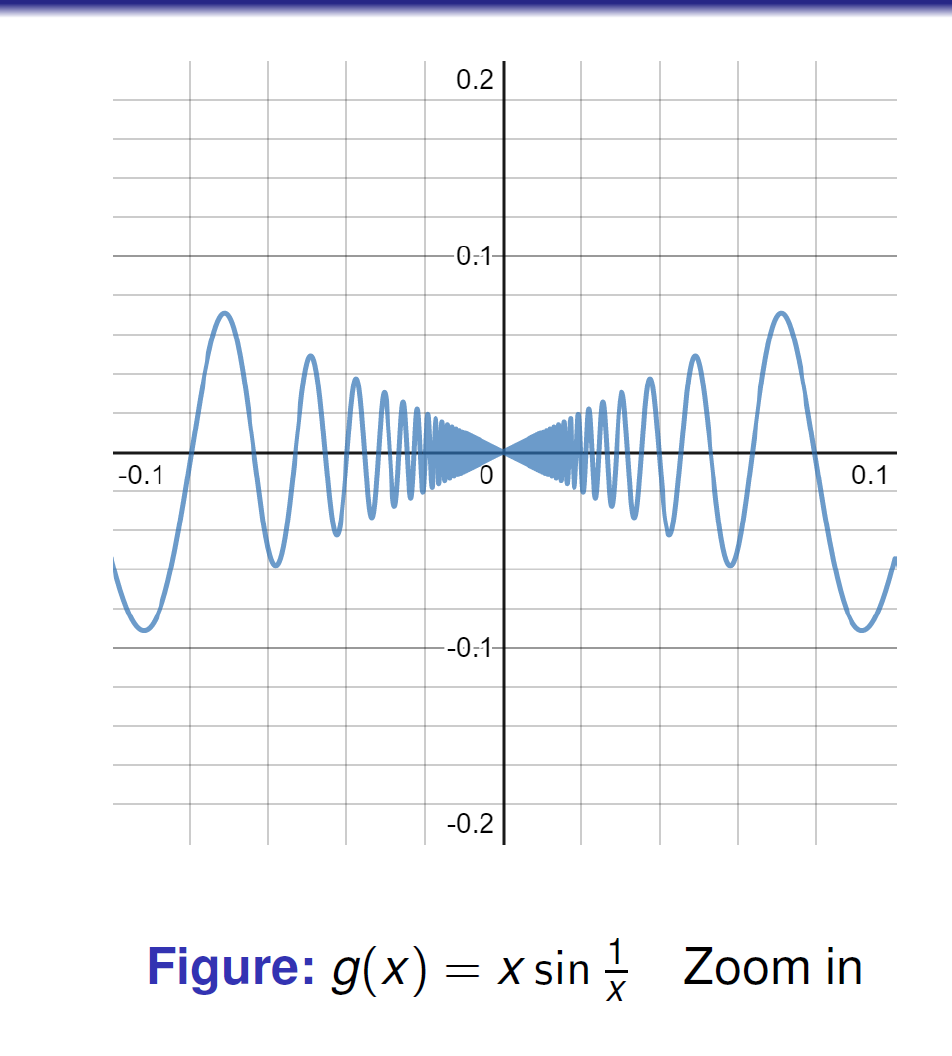
\includegraphics[width=0.65\textwidth]{image-1.png}
\end{center}

Useful estimates:
\[
|f(x)|\le |x|^2,\qquad |g(x)|\le |x|.
\]

Therefore:
\[
\lim_{x\to0}f(x)=\underline{\hspace{2cm}},\qquad
\lim_{x\to0}g(x)=\underline{\hspace{2cm}}.
\]

My takeaway:
\begin{quote}
If $x$ gets close to 0, keeping $x\ne0$, $f(x)$ approaches 0 with error $\leq |x|^2$; $g(x)$ approaches 0 with error $\leq |x|$.
\end{quote}

\subsubsection*{Example 2: Average speed and instantaneous speed}
\textbf{Average speed:}
\[
\frac{\Delta s}{\Delta t}
=\frac{f(t_2)-f(t_1)}{t_2-t_1}.
\]

With $h=t_2-t_1$:
\[
\frac{f(t_1+h)-f(t_1)}{h}.
\]

\textbf{Instantaneous speed at $t_0$:}
\[
v(t_0)=\lim_{h\to0}\frac{f(t_0+h)-f(t_0)}{h}
=\lim_{t\to t_0}\frac{f(t)-f(t_0)}{t-t_0}.
\]

\subsection*{Informal definition of limit}
\begin{quote}
Assume $f(x)$ is defined on an open interval about $c$, except possibly at $c$ itself. If $f(x)$ is arbitrarily close to $L$ for all $x$ sufficiently close to $c$ other than $c$ itself, then
\[
\lim_{x\to c}f(x)=L.
\]
This is read ``the limit of $f(x)$ as $x$ approaches $c$ is $L$.''
\end{quote}

\subsection*{3. Limit calculation techniques}
\subsubsection*{Algebraic simplification}
\[
\lim_{x\to1}\frac{x^2-1}{x-1}
=\lim_{x\to1}(x+1)
=\underline{\hspace{2cm}}.
\]

\subsubsection*{Rationalizing the denominator}
\[
\lim_{x\to1}\frac{\sqrt{x}-1}{x-1}
=\lim_{x\to1}\frac{1}{\sqrt{x}+1}
=\underline{\hspace{2cm}}.
\]

\textbf{Remark:} Simplification when calculating limits.

\textbf{General strategy:}
\begin{enumerate}
	\item Check direct substitution.
	\item Factor or rationalize if necessary.
	\item Simplify, then evaluate the limit.
\end{enumerate}

\subsection*{Class 2: Describing the behavior of a function as $x\to0$}

\textbf{1. Jump}
\begin{center}
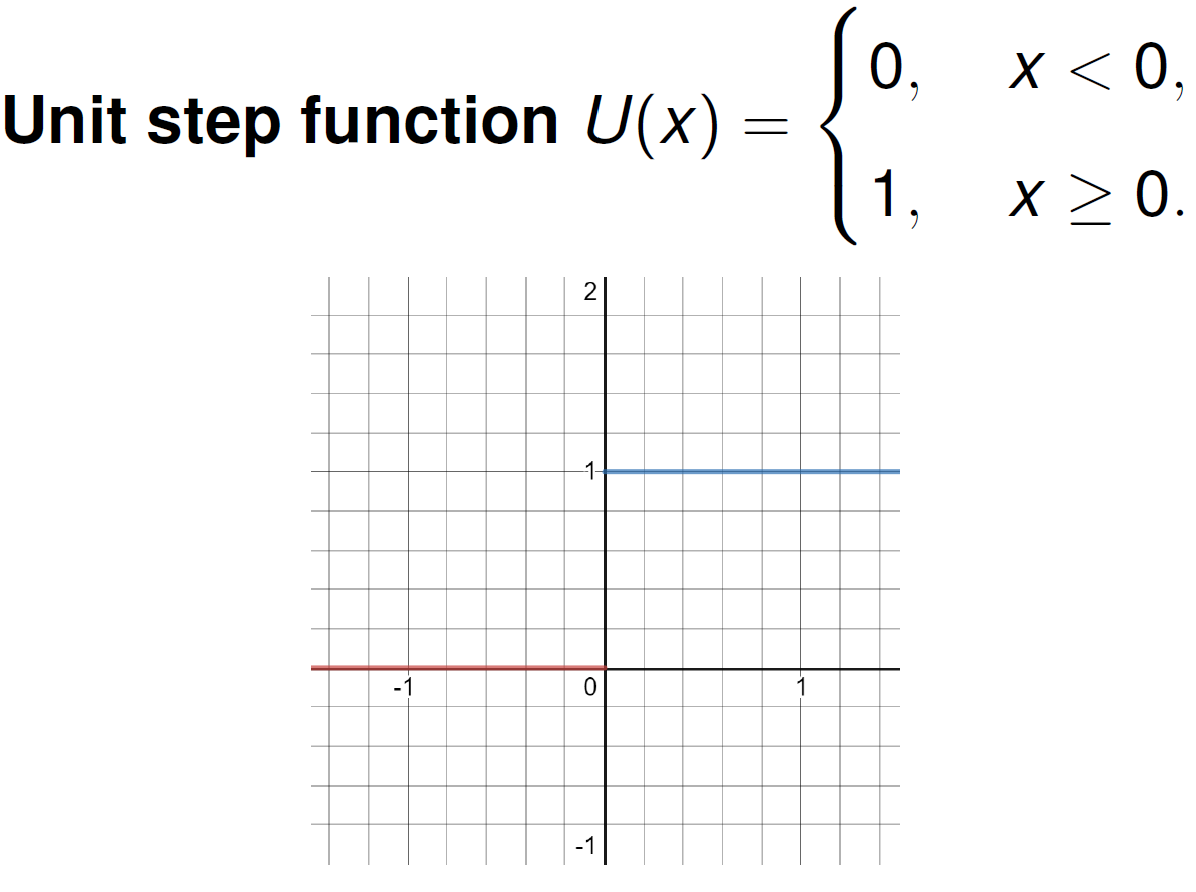
\includegraphics[width=0.65\textwidth]{image-2.png}
\end{center}

\textbf{2. Unbounded}
\begin{center}
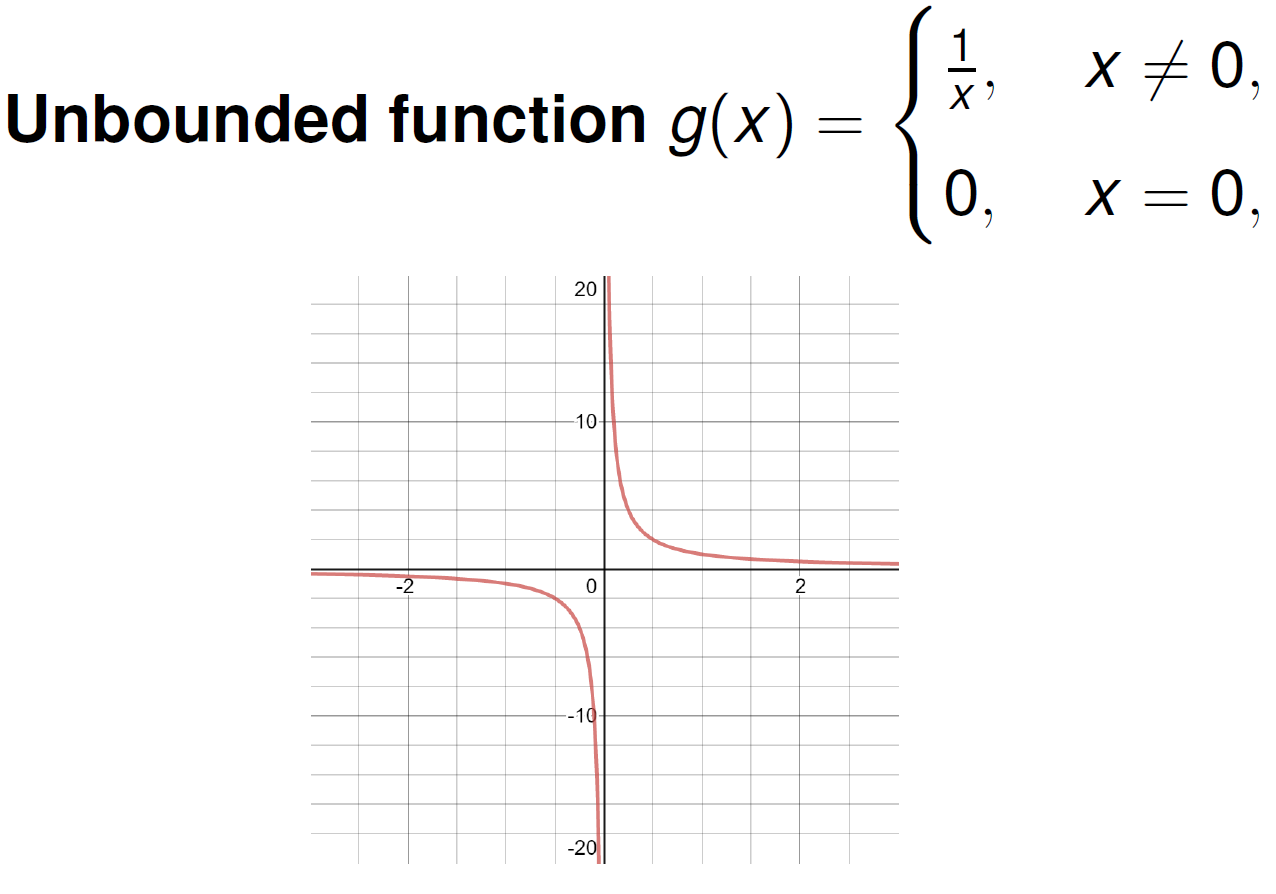
\includegraphics[width=0.65\textwidth]{image-3.png}
\end{center}

\textbf{3. Oscillation}
\begin{center}
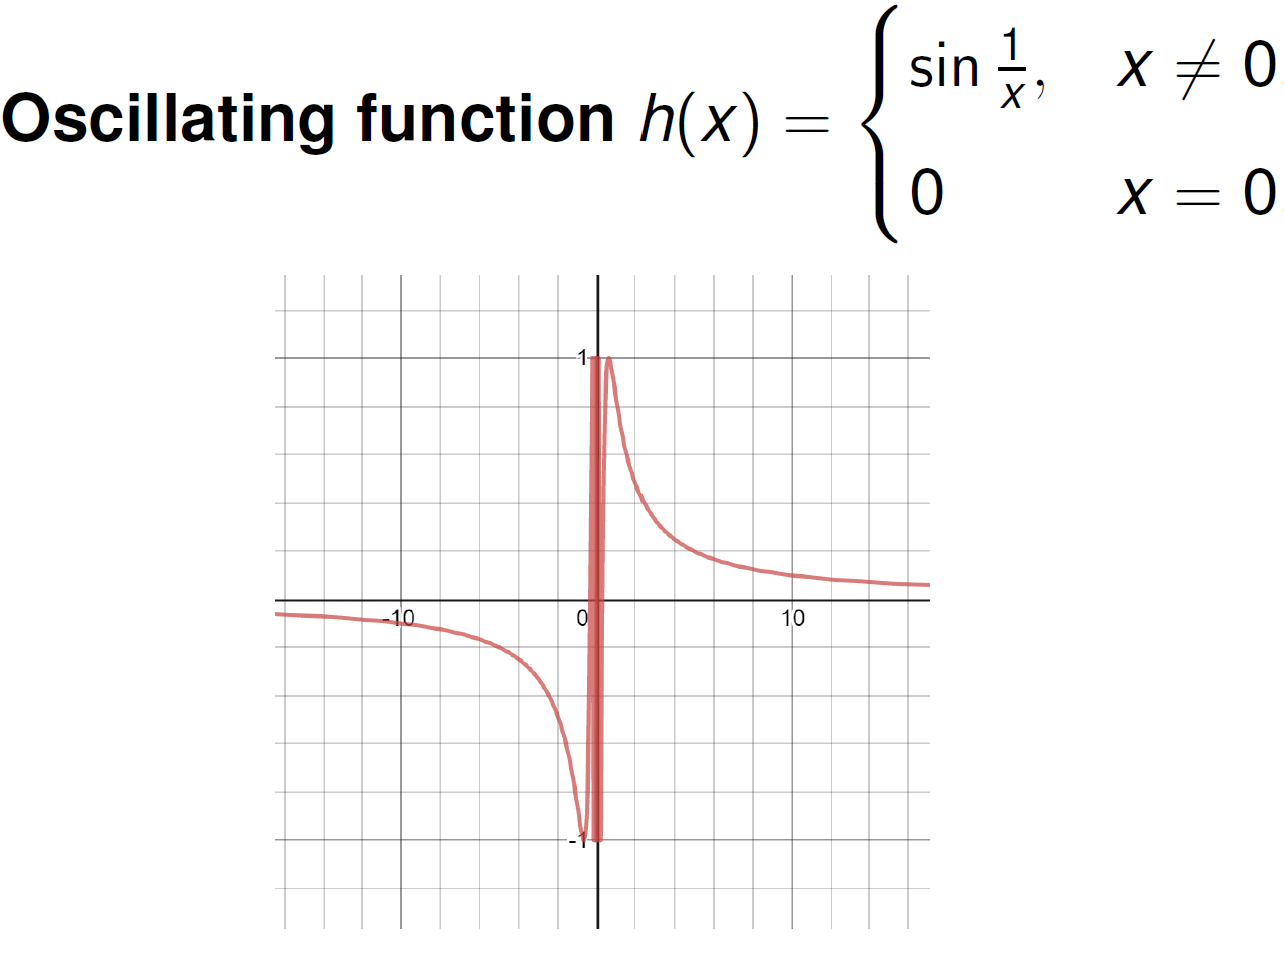
\includegraphics[width=0.65\textwidth]{image-4.png}
\end{center}

\subsection*{4. When a limit does not exist}
\begin{center}
\begin{tabular}{p{0.18\textwidth} p{0.48\textwidth} p{0.22\textwidth}}
	\textbf{Type} & \textbf{What happens near the point?} & \textbf{Example} \\
	\hline
	Jump & Left and right sides approach different values & Unit step function \\
	Unbounded & Function values grow without bound & $1/x$ near 0 \\
	Oscillation & Values do not approach one fixed number & $\sin(1/x)$ near 0 
\end{tabular}
\end{center}

\subsection*{A few words}

\begin{quote}
	I will take notes in class every time, and I will post them to my personal website. The notes will include the main points of the lecture, and I will try to make them as clear as possible. However, I will not be able to include all the details, so please make sure to attend the lectures. Also, I will not be writing down every single example, so please make sure to read the textbook and do the exercises.
\end{quote}

\section*{Lecture 2}

\subsection*{Definition of limit (Informal)}
\[
g(x)=
\begin{cases}
2x, & \text{if } x\ne4,\\
0, & \text{if } x=4.
\end{cases}
\]

By the informal description of a limit: if $x$ gets sufficiently close to $4$, but is not equal to $4$, then $g(x)$ gets arbitrarily close to $8$.

We need to show that the gap between $g(x)$ and $L=8$, namely $|g(x)-8|$, can be made as small as we choose if $x$ is kept close enough to $c=4$, but is not equal to $4$.

\subsection*{Definition}

Let $f(x)$ be defined on an open interval $I$ about $c$, except possibly at $c$ itself. We say that the limit of $f(x)$ as $x$ approaches $c$ is the number $L$, and write
\[
\lim_{x\to c}f(x)=L,
\]
if, for every $\varepsilon>0$, there exists a corresponding $\delta>0$ such that
\[
|f(x)-L|<\varepsilon
\quad\text{whenever }x\in I\text{ and }0<|x-c|<\delta.
\]

\subsection*{Simpler writing}

We say $\lim_{x\to c}f(x)=L$ if, for any $\varepsilon>0$, there exists $\delta>0$ such that
\[
\text{if }x\in I,\quad 0<|x-c|<\delta,
\quad\text{then }|f(x)-L|<\varepsilon.
\]

\subsection*{Personal interpretation}

\begin{itemize}
\item $\varepsilon$: how close we require $f(x)$ to be to $L$.
\item $\delta$: how close $x$ needs to be to $c$ in order to satisfy that requirement.
\item $|f(x)-L|<\varepsilon$: $f(x)$ lies within an $\varepsilon$-neighborhood of $L$.
\item $0<|x-c|<\delta$: $x$ lies within a $\delta$-neighborhood of $c$, but $x\ne c$.
\end{itemize}

The key idea is
\[
\boxed{\text{Given any }\varepsilon>0,\text{ we can find a }\delta>0}
\]
such that
\[
x\text{ is sufficiently close to }c
\quad\Longrightarrow\quad
f(x)\text{ is within }\varepsilon\text{ of }L.
\]

In other words, $\varepsilon$ is the required accuracy for the output, while $\delta$ is how much accuracy we need for the input.

Thus, the $\varepsilon$-$\delta$ definition gives a precise mathematical meaning to the intuitive statement: if $x$ is sufficiently close to $c$, then $f(x)$ is sufficiently close to $L$.

\subsection*{Useful remarks}

We shall often use the following arguments:
\begin{enumerate}[label=(\roman*)]
\item Let $a$ be a real number. If, for every $\varepsilon>0$, we have $a\leq\varepsilon$, then $a\leq0$.
\item Let $a$ be a real number. If, for every $\varepsilon>0$, we have
\[
-\varepsilon\leq a\leq\varepsilon,
\]
then $a=0$.
\end{enumerate}

\subsection*{Example: revisiting $g(x)$}

Consider
\[
g(x)=
\begin{cases}
2x, & \text{if }x\ne4,\\
0, & \text{if }x=4.
\end{cases}
\]

Show that
\[
\lim_{x\to4}g(x)=8.
\]

\textbf{Analysis.} For every $\varepsilon>0$, we need
\[
|g(x)-8|=|2x-8|<\varepsilon,
\qquad x\ne4,
\]
which requires
\[
0<|x-4|<\frac{\varepsilon}{2}.
\]

\textbf{Proof.} Given arbitrary $\varepsilon>0$, take
\[
\delta=\frac{\varepsilon}{2}.
\]
Then
\[
|g(x)-8|=|2x-8|=2|x-4|<2\delta=\varepsilon
\]
whenever $0<|x-4|<\delta$. By the definition of limit,
\[
\lim_{x\to4}g(x)=8.
\]

\subsection*{Exercise}

Prove that
\[
\lim_{x\to1}\frac{1}{x}=1.
\]

\textbf{Hint.} Restrict $x$ by taking $x>\frac12$. Then
\[
\left|\frac{1}{x}-1\right|=\frac{|x-1|}{|x|}<2|x-1|.
\]

\subsection*{Exercise 1.1.5 revisited}

Using the definition of limit, prove that the following functions have no
limit as $x\to0$.

\subsubsection*{(a)}
\[
U(x)=
\begin{cases}
0, & x<0,\\
1, & x\geq0.
\end{cases}
\]

\subsubsection*{(b)}
\[
g(x)=
\begin{cases}
\dfrac{1}{x}, & x\ne0,\\
0, & x=0.
\end{cases}
\]

\subsubsection*{(c)}
\[
f(x)=
\begin{cases}
0, & x\leq0,\\
\sin\dfrac{1}{x}, & x>0.
\end{cases}
\]

\textbf{Tip.} Suppose the limit exists and derive a contradiction.

\subsubsection*{For (b)}
Suppose
\[
\lim_{x\to0}\frac{1}{x}=L.
\]
Use the definition of the limit with $\varepsilon_0=1$.

\section*{Lecture 3}
\textbf{Date:} 2026.9.10

\subsection*{Theorem 1.1.3 (Limit Laws)}

Assume that
\[
\lim_{x\to c}f(x)=L
\qquad\text{and}\qquad
\lim_{x\to c}g(x)=M.
\]

\subsubsection*{(a) Sum Rule}
\[
\lim_{x\to c}\bigl(f(x)+g(x)\bigr)
=\lim_{x\to c}f(x)+\lim_{x\to c}g(x).
\]

\subsubsection*{(b) Product Rule}
\[
\lim_{x\to c}\bigl(f(x)\cdot g(x)\bigr)
=\lim_{x\to c}f(x)\cdot\lim_{x\to c}g(x).
\]

\subsubsection*{(c) Quotient Rule}

If $M\ne0$, then
\[
\lim_{x\to c}\frac{f(x)}{g(x)}
=\frac{\displaystyle\lim_{x\to c}f(x)}
{\displaystyle\lim_{x\to c}g(x)}.
\]

\subsection*{Remark: Does the Converse Hold?}

The Sum Rule requires that both limits on the right-hand side exist. In
general, the converse is false: the existence of
\[
\lim_{x\to c}(f(x)+g(x))
\]
does not imply that both $\lim_{x\to c}f(x)$ and $\lim_{x\to c}g(x)$ exist.

\subsubsection*{Counterexample}

Let
\[
f(x)=\sin\frac{1}{x},
\qquad
g(x)=-\sin\frac{1}{x}.
\]

Consider $x\to0$. Although
\[
\lim_{x\to0}\sin\frac{1}{x}
\]
does not exist, we have
\[
f(x)+g(x)=0.
\]
Therefore,
\[
\lim_{x\to0}(f(x)+g(x))=0
\]
exists. Thus,
\[
\boxed{
\lim(f+g)\text{ exists}
\not\Longrightarrow
\lim f,\lim g\text{ both exist}
}
\]

The problematic behavior of two functions can cancel each other out.

\subsection*{Exercise 1.1.9 (Limits of Polynomials)}

If
\[
P(x)=\sum_{k=0}^{n}a_kx^k
=a_nx^n+a_{n-1}x^{n-1}+\cdots+a_0,
\]
then
\[
\lim_{x\to c}P(x)
=\sum_{k=0}^{n}a_kc^k
=P(c).
\]

\subsection*{Exercise 1.1.10 (Limits of Rational Functions)}

If $P(x)$ and $Q(x)$ are polynomials and $Q(c)\ne0$, then
\[
\lim_{x\to c}\frac{P(x)}{Q(x)}=\frac{P(c)}{Q(c)}.
\]

\subsection*{Theorem 1.1.4 (The Sandwich Theorem)}

Suppose that
\[
g(x)\leq f(x)\leq h(x)
\]
for all $x$ in some open interval containing $c$, except possibly at $x=c$.
Suppose also that
\[
\lim_{x\to c}g(x)=\lim_{x\to c}h(x)=L.
\]
Then
\[
\lim_{x\to c}f(x)=L.
\]
\begin{center}
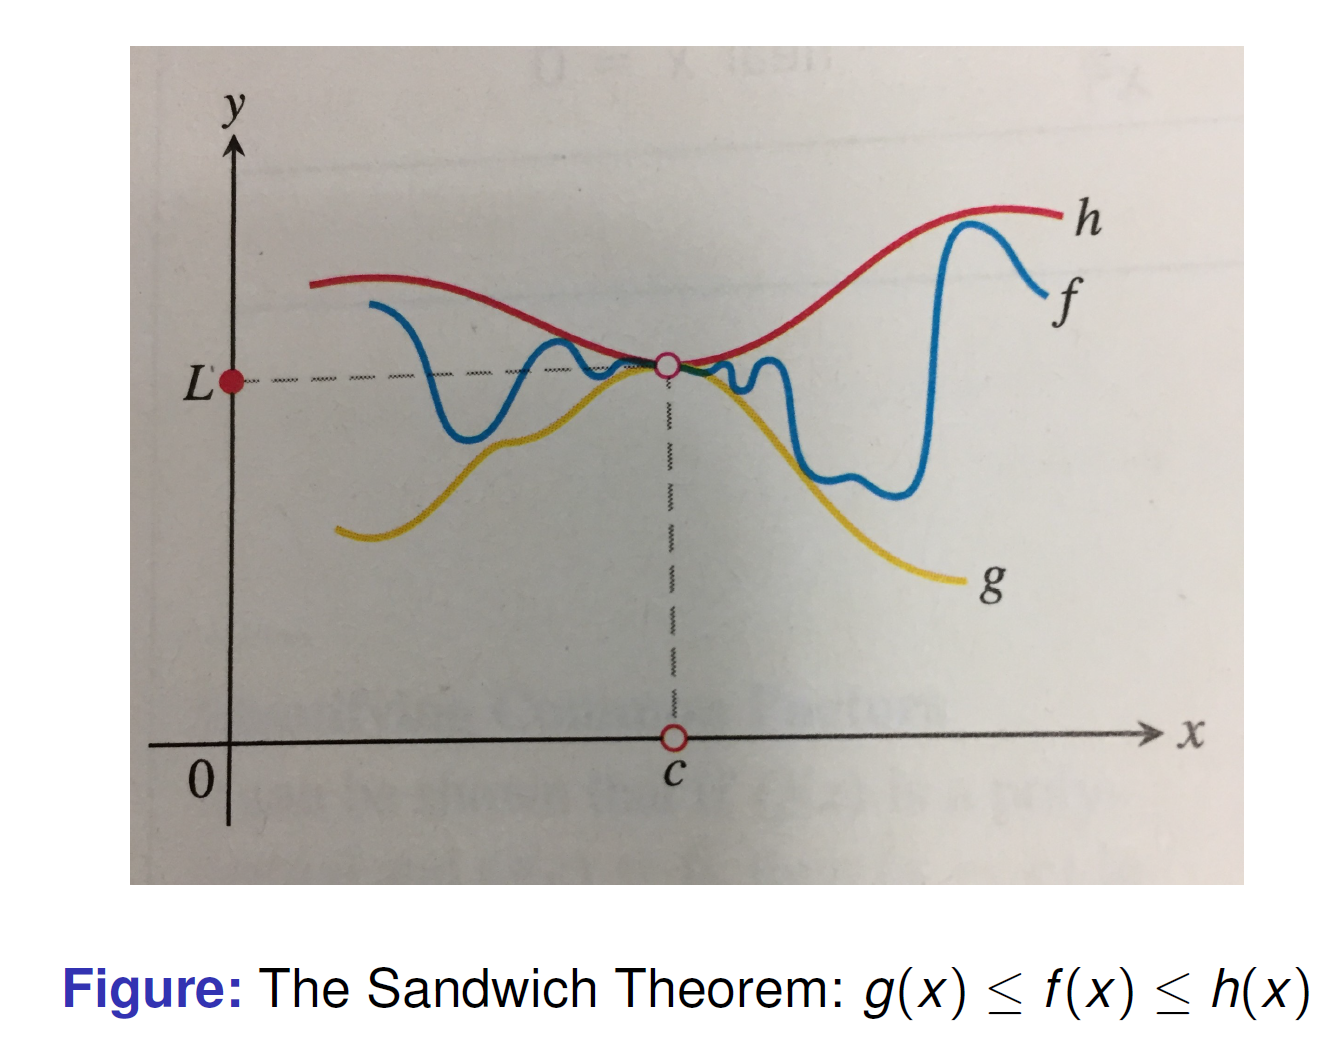
\includegraphics[width=0.65\textwidth]{image-5.png}
\end{center}

\subsection*{Exercise 1.1.12}

Assume $I$ is an open interval, $c\in I$, and
\[
f(x)\leq b
\qquad\text{for all }x\in I\setminus\{c\}.
\]
Then
\[
\lim_{x\to c}f(x)\leq b,
\]
provided the limit exists.

\subsection*{Exercise 1.1.13 (Order-preserving Property of Limits)}

If
\[
f(x)\leq g(x)
\]
for all $x$ in some open interval containing $c$, except possibly at $x=c$,
and both limits exist, then
\[
\lim_{x\to c}f(x)\leq\lim_{x\to c}g(x).
\]

Limits preserve the non-strict inequality $\leq$, but may not preserve the
strict inequality $<$. For example, let
\[
f(x)=x^2,
\qquad g(x)=2x^2.
\]
For $x\ne0$, $f(x)<g(x)$, but
\[
\lim_{x\to0}x^2=\lim_{x\to0}2x^2=0.
\]

\subsection*{Lemma 1.1.5}

For $\theta$ measured in radians,
\[
-|\theta|\leq\sin\theta\leq|\theta|,
\qquad
-|\theta|\leq1-\cos\theta\leq|\theta|.
\]
In particular, for $0<\theta\leq\dfrac{\pi}{2}$,
\[
0<\sin\theta<\theta.
\]
\begin{center}
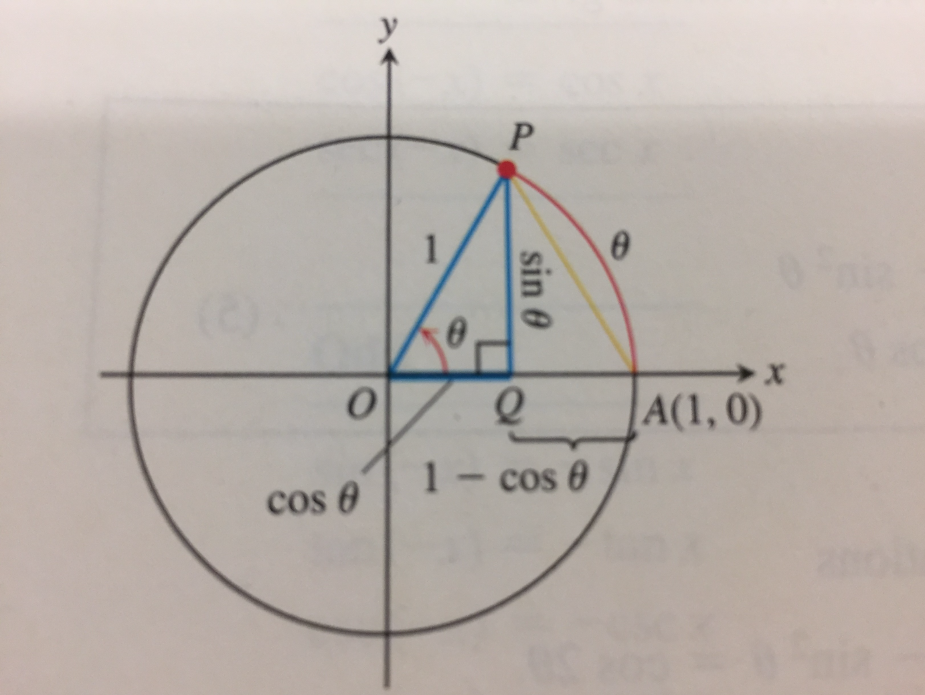
\includegraphics[width=0.65\textwidth]{image-7.png}
\end{center}

\subsection*{One-sided Limits}

\subsubsection*{Left-hand limit}
\[
\lim_{x\to c^-}f(x)=L
\]
if, for every $\varepsilon>0$, there exists $\delta>0$ such that
\[
c-\delta<x<c
\quad\Longrightarrow\quad
|f(x)-L|<\varepsilon.
\]

\subsubsection*{Right-hand limit}
\[
\lim_{x\to c^+}f(x)=L
\]
if, for every $\varepsilon>0$, there exists $\delta>0$ such that
\[
c<x<c+\delta
\quad\Longrightarrow\quad
|f(x)-L|<\varepsilon.
\]

The two-sided limit exists if and only if the one-sided limits both exist
and are equal:
\[
\lim_{x\to c}f(x)=L
\quad\Longleftrightarrow\quad
\lim_{x\to c^-}f(x)=\lim_{x\to c^+}f(x)=L.
\]

\subsubsection*{Examples at $x\to0$}

\paragraph{Example 1: The $0$-$1$ step function.}
\[
U(x)=
\begin{cases}
0, & x<0,\\
1, & x\geq0.
\end{cases}
\]
Then
\[
\lim_{x\to0^-}U(x)=0,
\qquad
\lim_{x\to0^+}U(x)=1,
\]
so the two-sided limit does not exist.

\paragraph{Example 2: The function $1/x$.}
\[
\lim_{x\to0^-}\frac{1}{x}=-\infty,
\qquad
\lim_{x\to0^+}\frac{1}{x}=+\infty.
\]
Thus, $1/x$ has no finite two-sided limit at $0$.

\paragraph{Example 3: The oscillating function $\sin(1/x)$.}
\[
\lim_{x\to0^-}\sin\frac{1}{x}
\quad\text{and}\quad
\lim_{x\to0^+}\sin\frac{1}{x}
\]
both do not exist.

\paragraph{The density of $\mathbb{Q}$ in $\mathbb{R}$.}

We say that $\mathbb{Q}$ is dense in $\mathbb{R}$ if every non-empty open
interval contains a rational number. For any $a,b\in\mathbb{R}$ with $a<b$,
there exists $q\in\mathbb{Q}$ such that
\[
a<q<b.
\]
Equivalently, for every $x\in\mathbb{R}$ and every $\varepsilon>0$, there
exists $q\in\mathbb{Q}$ such that
\[
|q-x|<\varepsilon.
\]
The irrational numbers are also dense in $\mathbb{R}$.

\paragraph{Example 4: The Dirichlet function.}
\[
D(x)=
\begin{cases}
1, & x\in\mathbb{Q},\\
0, & x\in\mathbb{R}\setminus\mathbb{Q}.
\end{cases}
\]
Every interval to the left or right of $0$ contains both rational and
irrational numbers. Hence,
\[
\lim_{x\to0^-}D(x)
\quad\text{and}\quad
\lim_{x\to0^+}D(x)
\]
both do not exist.

\subsection*{Theorem 1.1.6}

Suppose that $f(x)$ is defined on an open interval containing $c$, except
possibly at $c$ itself. Then $f(x)$ has a limit as $x$ approaches $c$ if and
only if its left-hand and right-hand limits both exist and are equal:
\[
\lim_{x\to c}f(x)=L
\quad\Longleftrightarrow\quad
\lim_{x\to c^-}f(x)=\lim_{x\to c^+}f(x)=L.
\]

\subsubsection*{Proof}

If $\lim_{x\to c}f(x)=L$, the $\varepsilon$-$\delta$ condition immediately
implies the same estimate for $x<c$ and for $x>c$. Therefore both one-sided
limits equal $L$.

Conversely, suppose both one-sided limits equal $L$. Given $\varepsilon>0$,
choose $\delta_1,\delta_2>0$ from the left- and right-hand definitions and
let
\[
\delta=\min\{\delta_1,\delta_2\}.
\]
If $0<|x-c|<\delta$, then either $c-\delta<x<c$ or
$c<x<c+\delta$. In either case,
\[
|f(x)-L|<\varepsilon.
\]
Thus $\lim_{x\to c}f(x)=L$.

\subsection*{Theorem 1.1.7}

For $\theta$ measured in radians,
\[
\lim_{\theta\to0}\frac{\sin\theta}{\theta}=1.
\]
\begin{center}
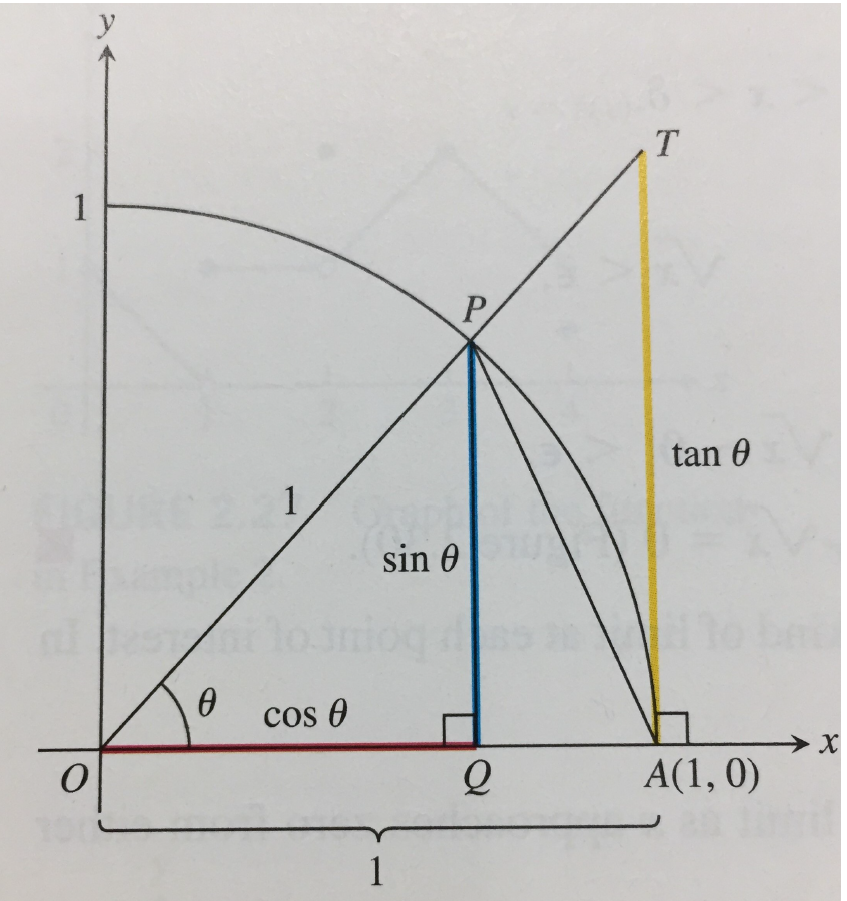
\includegraphics[width=0.65\textwidth]{image-8.png}
\end{center}

\subsubsection*{Proof}

For $0<\theta<\dfrac{\pi}{2}$,
\[
\cos\theta\leq\frac{\sin\theta}{\theta}\leq1.
\]
Since $\lim_{\theta\to0}\cos\theta=1$, the Sandwich Theorem gives
\[
\lim_{\theta\to0^+}\frac{\sin\theta}{\theta}=1.
\]
For $\theta<0$,
\[
\frac{\sin\theta}{\theta}
=\frac{\sin(-\theta)}{-\theta},
\]
so the left-hand limit is also $1$. Therefore,
\[
\boxed{\displaystyle\lim_{\theta\to0}\frac{\sin\theta}{\theta}=1}.
\]

\subsubsection*{Consequences}

For any constant $k\ne0$,
\[
\lim_{\theta\to0}\frac{\sin(k\theta)}{\theta}
=k\lim_{\theta\to0}\frac{\sin(k\theta)}{k\theta}=k.
\]
Also,
\[
\lim_{x\to0}\frac{\sin(\sin x)}{\sin x}=1,
\]
and, for $n$ nested sine functions,
\[
\lim_{x\to0}
\frac{\sin\bigl(\sin(\cdots\sin x\cdots)\bigr)}{x}=1.
\]

\subsubsection*{Proof of $\displaystyle\lim_{x\to0}\frac{\sin(\sin x)}{x}=1$}

Since $\lim_{x\to0}\sin x=0$, Theorem 1.1.7 gives
\[
\lim_{x\to0}\frac{\sin(\sin x)}{\sin x}=1.
\]
Moreover,
\[
\frac{\sin(\sin x)}{x}
=\frac{\sin(\sin x)}{\sin x}\cdot\frac{\sin x}{x}.
\]
Therefore,
\[
\begin{aligned}
\lim_{x\to0}\frac{\sin(\sin x)}{x}
&=\left(\lim_{x\to0}\frac{\sin(\sin x)}{\sin x}\right)
\left(\lim_{x\to0}\frac{\sin x}{x}\right)\\
&=1\cdot1=1.
\end{aligned}
\]

\section*{Lecture 4}

\subsection*{Example 1.1.19}
\[
f(x)=
\begin{cases}
x, & x<0,\\
1, & 0\leq x<1,\\
2, & x=1,\\
x, & x>1.
\end{cases}
\]
\begin{center}
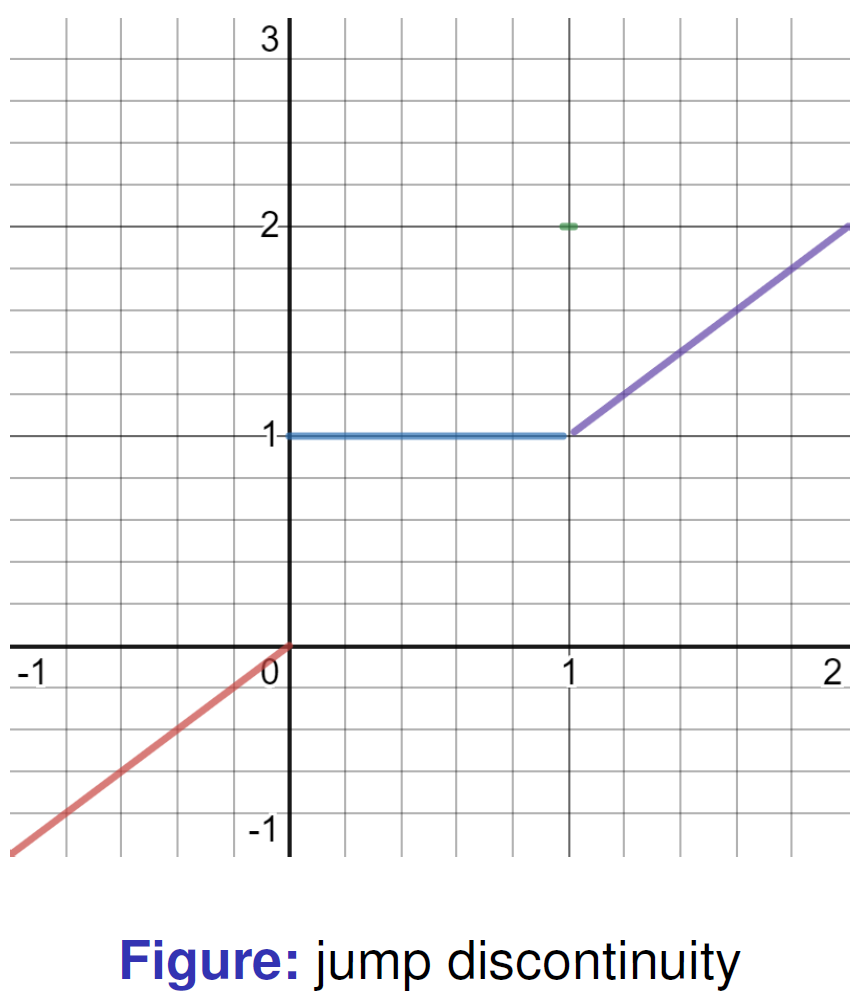
\includegraphics[width=0.65\textwidth]{image-9.png}
\end{center}

\subsection*{Definition 1.1.8 (Continuity at a Point)}

Let $c$ be a real number that is either an interior point or an endpoint of
an interval in the domain of $f$.

\subsubsection*{(a) Interior point}

$f$ is continuous at $c$ if
\[
\lim_{x\to c}f(x)=f(c).
\]

\subsubsection*{(b) Right-continuity}

$f$ is right-continuous at $c$ (or continuous from the right) if
\[
\lim_{x\to c^+}f(x)=f(c).
\]

\subsubsection*{(c) Left-continuity}

$f$ is left-continuous at $c$ (or continuous from the left) if
\[
\lim_{x\to c^-}f(x)=f(c).
\]

\end{document}
